\documentclass[11pt,a4paper]{article}

\usepackage[margin=0.75in]{geometry}
\usepackage{xcolor}
\usepackage{amsmath,amssymb}
\usepackage{booktabs}
\usepackage{tabularx}
\usepackage{tcolorbox}
\usepackage{listings}
\usepackage{helvet}                  
\usepackage[scaled=0.95]{inconsolata} 
\usepackage{graphicx}
\usepackage{float}
\usepackage{tikz}
\usepackage{hyperref}
\lstdefinestyle{cppstyle}{
    language=C++,
    basicstyle=\ttfamily\small,
    keywordstyle=\color{blue}\bfseries,
    stringstyle=\color{red},
    commentstyle=\color{gray}\itshape,
    numbers=left,
    numberstyle=\tiny\color{gray},
    stepnumber=1,
    numbersep=8pt,
    tabsize=4,
    showspaces=false,
    showstringspaces=false,
    breaklines=true,
    frame=single
}

\lstset{style=cppstyle}
\usetikzlibrary{positioning, arrows.meta, calc}

\hypersetup{
    colorlinks=true,
    urlcolor=blue
}

\title{Digital Clock}
\author{
  \textbf{Arjun R Iyengar} \\
  \small ee26btech11202\\
  \and
  \textbf{Arya Sudhirkumar Neel} \\
  \small ee26btech11203\\ \\}
\date{August 2026}
\begin{document}

\maketitle

\begin{center}
\section*{Phase 1: Learning the Theory and Connections}
\end{center}

\begin{itemize}
    \item The project was begun by learning the theory about binary operations, how decimal numbers can be converted into binary, and how each output binary digit can be expressed as a function of the inputs. We learnt the Karnaugh Maps(K-Maps) method for generating the functions and using this to increment(or decrement) the digits in the displays of the clock. We learnt the basics of coding in arduino, and the basic functions like pinMode, digitalWrite, millis, digitalRead etc.
    \item The components for building the clock include: Arduino Uno, IC 7447, Seven Segment Display(Common Anode), Breadboard, Jumper Wires, Resistors, Push Buttons
    \item In the next step, we learnt the purpose of using the IC 7447:    \begin{enumerate}
    \item It translates 4-bit Binary Coded Decimal (BCD) values (0000 to 1001) from the Arduino into the specific combinations of 7 segment lines (a–g) needed to display digits 0–9. Without it, the software code would have to manually calculate and output individual bit patterns for every single display update.
    \item The display receives those 7 segment signals and lights up the corresponding LED lines. At the same instant, the Arduino powers the common anode pin (D4–D9) of the targeted digit to turn it on.
   
that appears continuous.
    \end{enumerate}
    \item Understanding multiplexing:
    \begin{enumerate}
        \item Without multiplexing, every single digit display must be wired independently so it can receive its own unique data continuously.
        \item Multiplexing connects all display digits to the exact same 4-wire data bus, cutting down hardware drastically. We then add 1 extra "digit select" control pin per display to switch power ON or OFF to each digit individually.
         \item Persistence of Vision: Each digit is displayed for $1$ms, creating a fast alternating effect:
         \begin{align*}
         t_{\text{digit}}=0.001s \implies t_{\text{cycle}}=0.006s \\
         f_{\text{refresh}}= 1/t_{\text{cycle}} = 166.67 hz
         \end{align*}
         As this frequency is much higher than 60hz, our eyes are unable to perceive the individual displays turning ON and OFF sequentially.
    \end{enumerate}
    \item Understanding the connections to be made:
\begin{figure}[H]
\centering
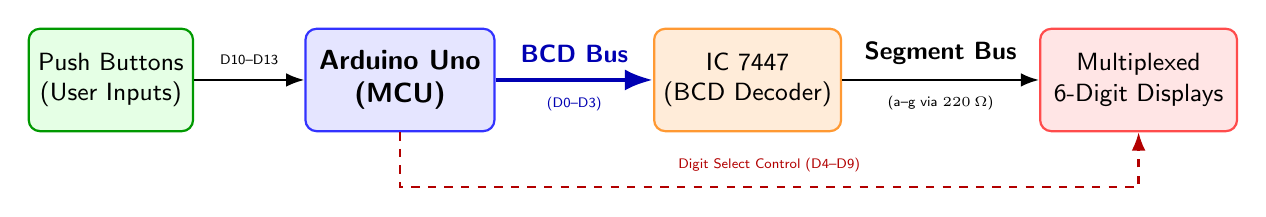
\begin{tikzpicture}[
    % Increased horizontal node spacing to prevent label crowding
    node distance=1.0cm and 2.4cm,
    % Block Styles
    block/.style={rectangle, draw=blue!80, fill=blue!10, thick, rounded corners, minimum width=2.4cm, minimum height=1.3cm, align=center, font=\sffamily\bfseries},
    input/.style={rectangle, draw=green!60!black, fill=green!10, thick, rounded corners, minimum width=2.0cm, minimum height=1.3cm, align=center, font=\sffamily\small},
    ic/.style={rectangle, draw=orange!80, fill=orange!15, thick, rounded corners, minimum width=2.2cm, minimum height=1.3cm, align=center, font=\sffamily\small},
    display/.style={rectangle, draw=red!70, fill=red!10, thick, rounded corners, minimum width=2.5cm, minimum height=1.3cm, align=center, font=\sffamily\small},
    % Line & Arrow Styles
    bus/.style={draw, -Latex, ultra thick, color=blue!70!black},
    line/.style={draw, -Latex, thick, color=black},
    enable/.style={draw, -Latex, thick, color=red!70!black, dashed}
]

    % Nodes
    \node [input] (buttons) {Push Buttons\\(User Inputs)};
    \node [block, right=1.4cm of buttons] (arduino) {Arduino Uno\\(MCU)};
    \node [ic, right=2.0cm of arduino] (decoder) {IC 7447\\(BCD Decoder)};
    \node [display, right=2.5cm of decoder] (displays) {Multiplexed\\6-Digit Displays};

    % Connections / Flow
    \draw [line] (buttons) -- node[above=2pt, font=\tiny\sffamily] {D10--D13} (arduino);
    
    % Core Flow: Arduino -> BCD Bus -> IC 7447 -> Segment Bus -> Displays
    \draw [bus] (arduino) -- node[above=2pt, font=\small\sffamily\bfseries] {BCD Bus} node[below=2pt, font=\tiny\sffamily] {(D0--D3)} (decoder);
    
    \draw [line] (decoder) -- node[above=2pt, font=\small\sffamily\bfseries] {Segment Bus} node[below=2pt, font=\tiny\sffamily] {(a--g via $220\,\Omega$)} (displays);

    % Multiplex Digit Select Control Loop
    \draw [enable] (arduino.south) -- ++(0,-0.7) -| node[near start, above=2pt, font=\tiny\sffamily] {Digit Select Control (D4--D9)} (displays.south);

\end{tikzpicture}
\caption{High-Level System Overview Block Diagram}
\label{fig:system_overview}
\end{figure}
    
    
    
\end{itemize}
\begin{center}
    \section*{Phase 2: Making the First Set of Connections}
\end{center}

\noindent The following set of connections were made to get a feel of the process, and to test a single display(display 6)
\begin{figure}[H]
    \centering
    \includegraphics[width=0.75\linewidth]{figs/Initial_connections.jpeg}
    \caption{First set of Connections}
    \label{fig:placeholder}
\end{figure}

{\centering\section*{Phase 3: Coding and debugging for first display}}

\subsection*{Code}
\noindent{We began writing the code, and got used to the logic of the code, using the pinMode, digitalWrite functions and setting up the functions to display the digits and increment them. } 
\subsection*{Fixing the errors}
\begin{enumerate}
    \item The first attempt was to change the display to check if it was faulty, which did not work, which was followed by checking for loose connections and changing wires, which also failed, as all connections were correct.
    \item Upon researching, the solution that we found was that the pin 4 of the IC 7447 needed to be connected to the 5V rail on the breadboard. This was needed because even though technically, the clock might appear to work temporarily because the 7447 naturally defaults to a HIGH logic state when the pins are left disconnected. However, it will not work reliably and will introduce erratic display bugs.\\
        Pin 4 ($\overline{\text{BI}}/\overline{\text{RBO}}$ — Blanking Input): When connected to GND (0V), this pin forcibly shuts OFF all 7 segments, ignoring whatever BCD number is being sent to the chip. Tying it to 5V disables forced blanking, keeping the display outputs active.
    \item Another change we made was changing the BCD input pins from D0-D3 to D2-D5, as the D0 and D1 pins are reserved for USB serial communication and uploading code, which caused errors upon uploading our code.
    
\end{enumerate}
\begin{figure}[H]
    \centering
    \includegraphics[width=0.75\linewidth]{figs/First_Display.jpeg}
    \caption{First Display Working}
    \label{fig:placeholder}
\end{figure}
\noindent {This was followed by testing all the common anode displays and verifying if each one of them counts the seconds from 0-9, so that no error of the display being faulty in the future would be encountered.}
\begin{center}
    \section*{Phase 4: Adding all of the Displays}
\end{center}
\noindent {We decided to go step by step and make the connections for each display one by one, so that we can detect errors in each display, instead of finishing the connections to all displays}.

 
\begin{enumerate}

    \item Upon adding the second, display, we noticed that some segments(e and f) of the display were not lighting up as shown in the figure below:
\begin{figure}[H]
    \centering
    \includegraphics[width=0.75\linewidth]{figs/2displays_notworking.jpeg}
    \caption{Segment 'f' not lighting up for second display}
    \label{fig:placeholder}
\end{figure}
\item To fix the segment 'f', we fixed the loose connection issues, and for segment 'e', we realised that one column of the breadboard was not supporting correct flow of current, so we moved both the resistor and the jumper wire to another row, fixing the error.
\item No errors were encountered after adding the third display. We encountered another loose connection error upon adding and making the connections for the fourth display, which was fixed.
\begin{figure}[H]
    \centering
    \includegraphics[width=0.70\linewidth]{figs/4Displays.jpeg}
    \caption{Loose connection error}
    \label{fig:placeholder}
\end{figure}

\item{Next, we made the connections for the fifth and sixth segment. This was the progress after adding the fifth display}
\begin{figure}[H]
    \centering
    \includegraphics[width=0.75\linewidth]{figs/5_Displays.jpeg}
    \caption{Progress after five Displays}
    \label{fig:placeholder}
\end{figure}


\end{enumerate}
{\centering
    \section*{Phase 5: Adding the Buttons}
}
\noindent We figured out the mechanism behind which the buttons work,what connections were needed to be made and worked on what needed to be added to the code.
\begin{enumerate}
    \item The four buttons follow active-HIGH logic, with each button using a $10\text{k}\Omega$ pull-down resistor to guarantee clean $5\text{V}$ (HIGH) signals when pressed and $0\text{ V}$ (LOW) signals when released.
    \item One side of every button connects directly to the $+5\text{ V}$ power rail, while the opposite side connects to its designated Arduino digital input pin.
    \item While idle, the $10\text{k}\Omega$ resistor continuously drains stray current to Ground to hold the pin at $0\text{ V}$ (LOW). Connecting the other side of the switch to +5V creates a low-resistance path to power when pressed, overriding the $10\text{k}\Omega$ resistor and pulling the pin voltage cleanly up to $5\text{ V}$.
    \item The concept of {debouncing}: Pushing a tactile switch causes its metal contacts to physically bounce for 5–20 ms before establishing a steady connection. To avoid the pin state being read in this window, the millis function is utilised to debounce it.
\end{enumerate}
\noindent{Upon making the connections to the buttons, we noticed that the next digit selection button was working.}
\begin{enumerate}
    \item To identify the error we tried changing the arduino pins first and discovered the A0 pin to not function with the code.
    \item As the increment and 'next' buttons were still not working, upon trial and error, replacing one of the pause button wires, and changing the 'next' button fixed the issue.
\end{enumerate}
\noindent{However, we encountered an error where the number of hours was going above 23, to say 29}
\begin{figure}[H]
    \centering
    \includegraphics[width=0.75\linewidth]{figs/29_hours.jpeg}
    \caption{Enter Caption}
    \label{fig:placeholder}
\end{figure}
\begin{lstlisting}
case 4:
      A = !W5;
      B = (W5 && !X5 && !Z5) || (!W5 && X5);
      C = (!X5 && Y5) || (!W5 && Y5) || (W5 && X5 && !Y5);
      D = (!W5 && Z5) || (W5 && X5 && Y5);
      W5 = A; X5 = B; Y5 = C; Z5 = D;
      break;
// Increment code allowed Hours unit display  to go from 0-9 for any value of Hours tens display.
\end{lstlisting}
\begin{center} Incorrect Increment logic \end{center}
\begin{lstlisting}
case 4:
      if (X6 == 1) {
        if (Y5 || Z5){
          W5 = 0; X5 = 0; Y5 = 0; Z5 = 0;
        } else{
          A = !W5;
          B = (W5 && !X5) || (!W5 && X5);
          W5 = A; X5 = B; Y5 = 0; Z5 = 0;
        }
      } else {
        A = !W5;
        B = (W5 && !X5 && !Z5) || (!W5 && X5);
        C = (!X5 && Y5) || (!W5 && Y5) || (W5 && X5 && !Y5);
        D = (!W5 && Z5) || (W5 && X5 && Y5);
        W5 = A; X5 = B; Y5 = C; Z5 = D;
      }
      break;
// Fixed logic for increment code
\end{lstlisting}
\begin{center}Fixed Increment logic \end{center} 
\noindent The decrement logic also had the issue of displaying hours greater than 23,  which was fixed by changing the code.
\begin{figure}[H]
    \centering
    \includegraphics[width=0.75\linewidth]{figs/working_clock.jpeg}
    \caption{Working Clock}
    
    \label{fig:placeholder}
\end{figure}

\begin{center}
\noindent The video of the full working clock : \\ \url{https://www.youtube.com/watch?v=Ov-uN5F9GWs}
\end{center}

\end{document}
